\documentclass[a4paper,11pt]{article}

% ---------- Packages ----------
\usepackage[margin=2.5cm]{geometry}
\usepackage{amsmath, amssymb, amsthm, mathtools}
\usepackage{algorithm}
\usepackage{algpseudocode}
\usepackage{enumitem}
\usepackage{graphicx}
\usepackage{booktabs}
\usepackage{hyperref}
\usepackage{xcolor}

\usepackage{tikz}
\usetikzlibrary{automata,positioning,arrows.meta}

% ---------- Theorem Environments ----------
\newtheorem{theorem}{Theorem}
\newtheorem{lemma}{Lemma}
\newtheorem{definition}{Definition}
\newtheorem{proposition}{Proposition}
\newtheorem{corollary}{Corollary}

% ---------- Custom Commands ----------
\newcommand{\R}{\mathbb{R}}
\newcommand{\N}{\mathbb{N}}
\newcommand{\Z}{\mathbb{Z}}
\newcommand{\Alphabet}{\Sigma}
\newcommand{\eps}{\varepsilon}
\newcommand{\set}[1]{\left\{ #1 \right\}}
\newcommand{\abs}[1]{\left| #1 \right|}
\newcommand{\ceil}[1]{\left\lceil #1 \right\rceil}
\newcommand{\floor}[1]{\left\lfloor #1 \right\rfloor}

% ---------- Algorithm Style ----------
\algrenewcommand\algorithmicrequire{\textbf{Input:}}
\algrenewcommand\algorithmicensure{\textbf{Output:}}

% ---------- Title Info ----------
\title{\textbf{CSE2315 — Assignment 1}}
\author{Vlad Paun \\ 6152937}
\date{\today}

% ---------- Document ----------
\begin{document}

	\maketitle
	%\thispagestyle{empty}
	%\newpage

	\section{Exercise 1}
	Consider a language $L=\set{ok,a,bad,dab,abba,hi,\eps,acc,duck}$
	\subsection*{(a) Give a possible $\Alphabet$ such at $L \subseteq \Alphabet^*$}
	\[
	\Alphabet = \set{a,b,c,d,h,i,k,o,u}
	\]
	\subsection*{(b) Why is this only possible $\Alphabet$}
	Supposing this question is asking why this is the only possible \textbf{minimal} alphabet, the answer is that it must contain exactly the set of symbols that appear in the words in $L$, and that set is uniquely determined.
	\subsection*{(c) Give all words in $L$ in shortlex order}
	\[
	\eps,a,hi,okacc,bad,dab,abba,duck
	\]

	\section{Exercise 2}
	Consider the following claims (a) and (b). For each claim, verify whether it is true for arbitrary languages $L_1\subseteq\Alphabet^*_1$,$L_2\subseteq\Alphabet^*_2$,$L_3\subseteq\Alphabet^*_3$,$L_4\subseteq\Alphabet^*_4$. If a claim is true, give a proof; if it is not true, give a counterexample with an explanation how the counterexample shows the claim is false.
	\subsection*{(a) If $L_1\cup L_2 = L_3\cup L_4$, then $\Alphabet_1 \cup \Alphabet_2 = \Alphabet_3 \cup \Alphabet_4$}
	\textbf{FALSE.}\\
	Counterexample:
	\begin{align*}
	\Alphabet_1=\set{a,x},\Alphabet_2=\set{b},\Alphabet_3=\set{a,y},\Alphabet_4=\set{b}\\
	L_1=\set{a},L_2=\set{b},L_3=\set{a},L_4=\set{b}\\
	\\
	L_1\cup L_2 = L_3\cup L_4 = \set{a,b}\\
	\Alphabet_1 \cup \Alphabet_2 = \set{a,b,x} \neq \Alphabet_3 \cup \Alphabet_4 = \set{a,b,y}
	\end{align*}

	\subsection*{(b) If $L_1\cup L_2 \subseteq L_3\cap L_4$, then $L_1L_2 \subseteq L_3L_4$}
	\textbf{TRUE.}\\
	\begin{proof}
		From the first part of the implication, it follows that every word in $L_1$ and every word is $L_2$ is in both $L_3$ and $L_4$, so $\L_1 \subseteq L_3$ and $L_2 \subseteq L_4$\\
		Take an arbitrary word $w\in L_1L_2$. By definition of concatenation, we have $w=xy$ such that $x\in L_1$ and $y\in L_2$. From earlier, $x\in L_3$ and $y\in L_4$. Therefore, $w=xy\in L_3L_4$. Since w is arbitrary, it holds that $\forall w\in L_1L_2: w\in L_3L_4$. So $L_1L_2\subseteq L_3L_4.$
	\end{proof}


	\section{Exercise 3}
	Suppose we have an alphabet $\Alphabet = \set{a,b}$. Construct a DFA $M=(Q,\Alphabet,\delta,q_0,F )$ that recognizes the following language $L\subseteq \Alphabet^*$:
	\[
	L=\set{w|\text{each $b$ in $w$ is immediately preceeded by at least two $a$s and w ends with an $a$}}
	\]
	\subsection*{(a) Give the transition graph of $M$. Use no more than 6 states.}
	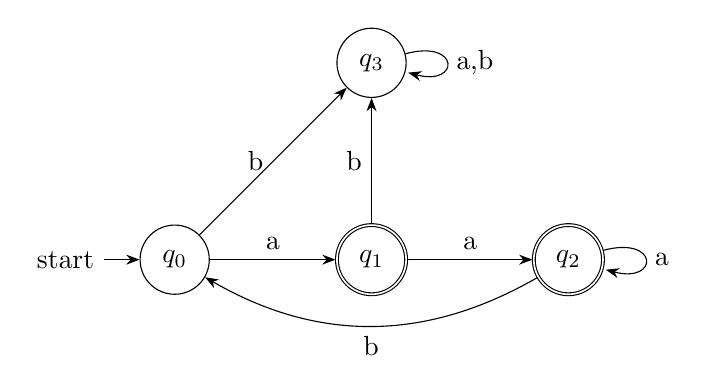
\begin{tikzpicture}[->, >=Stealth, auto, node distance=2.5cm]
		\node[initial,state] (q0) {$q_0$};
		\node[accepting,state] (q1) [right of=q0] {$q_1$};
		\node[accepting,state] (q2) [right of=q1] {$q_2$};
		\node[state] (q3) [above of=q1] {$q_3$};

		\path
		(q0) edge node {a} (q1)
		edge node[left] {b} (q3)
		(q1) edge node {a} (q2)
		edge node {b} (q3)
		(q2) edge[loop right] node {a} (q2)
		edge[bend left] node {b} (q0)
		(q3) edge[loop right] node {a,b} (q3);
	\end{tikzpicture}
	\subsection*{(b) Describe briefly how $M$ works.}
	Basically it counts if there s been at least 2 $a$s before a $b$. If not, the word is invalid so we go to a non-accepting state of $q_3$, which gets stuck there. If we get a $b$ in a valid position, we go back to the beginning thing. Also, to check that it ends in a, only $q_2$ and $q_3$ are valid.

	\section{Exercise 4}
	Consider the DFA $D=(\set{q_a,q_b,q_c},\set{0,1},\delta,q_a,\set{q_a})$, where $\delta$ is represented using the following transition table:
	\begin{tabular}{c|cc}
		  & 0     & 1     \\ \hline
	$q_a$ & $q_b$ & $q_a$ \\
	$q_b$ & $q_b$ & $q_c$ \\
	$q_c$ & $q_c$ & $q_a$ \\
	\end{tabular}
	\subsection*{(a) Give a transition diagram that corresponds to $D$.}
	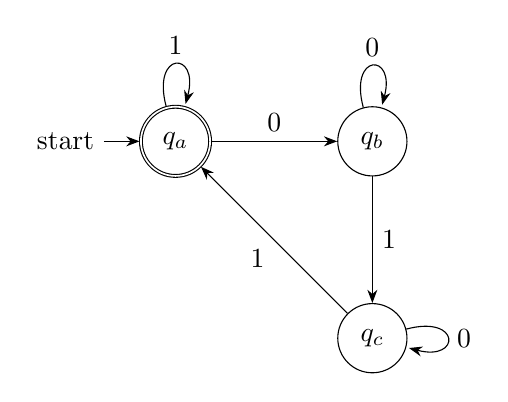
\begin{tikzpicture}[->, >=Stealth, auto, node distance=2.5cm]
		\node[initial,accepting,state] (qa) {$q_a$};
		\node[state] (qb) [right of=qa] {$q_b$};
		\node[state] (qc) [below of=qb] {$q_c$};

		\path
		(qa) edge node {0} (qb)
		edge [loop above] node {1} (qa)
		(qb) edge [loop above] node {0} (qb)
		edge node {1} (qc)
		(qc) edge [loop right] node {0} (qc)
		edge node {1} (qa);
	\end{tikzpicture}

	\subsection*{(b) Give a word $w$ of length 3 that is not in $D$ but is in $D'=(Q,\Alphabet,\delta,q_a,F\cup \set{q_c})$}
	\[010\]
	\subsection*{(c) Now imagine that we create a DFA $D''=(Q\cup Q_2,\Alphabet,\delta_1,q_a,F)$, what do we know about $\delta_2$?}
	$
	\delta_1(q,s) =
	\begin{cases}
		\delta(q,s)  & \text{if } q\in Q \\
		\delta_2(q,s) & \text{else}
	\end{cases}
	$ for some function $\delta_2:Q_2 \times \Alphabet \to Q \cup Q_2$. $Q \cap Q_2 = \emptyset$
	Every state in $Q_2$ must have a transition defined for all inputs, so in our case, they must have a transition for $0$ and for $1$. So the number of extra transitions is $2|Q_2|$
	\subsection*{(d)Describe as accurately as possible the relation between $L(D)$ and $L(D'')$ in terms of $\subset$,$\subseteq$,$=$ relations. Explain your answer.}
	\[
	L(D) = L(D'')
	\]

	The starting state of $D''$ is in $Q$, and all transitions in $\delta$, which cover all states in $Q$ always remain in $Q$. So therefore, it is impossible for an input to leave $Q$ and go into $Q_2$. Therefore, $D$ and $D''$ are basically equivalent, as they have the same set of reachable states and stuff.

	\section{Exercise 5}
	\section{Bonus Exercise}

\end{document}